\documentclass[aspectratio=169]{beamer}

\usepackage{fontspec}
\usepackage{polyglossia}
\usepackage{color}
\usepackage{listings}
\setdefaultlanguage{russian}
\usepackage{csquotes}
\usetheme{metropolis}
\metroset{background=light}
\metroset{sectionpage=none}
\metroset{numbering=fraction}

\definecolor{ssaublue}{RGB}{77,144,205}
\setbeamercolor{frametitle}{fg=white, bg=ssaublue}
\setbeamercolor{title separator}{fg=ssaublue}

\setmainfont[
    Path = ../fonts/elektratextpro/,
    Extension = .otf,
    UprightFont = elektratextpro,
    BoldFont = elektratextpro_bold,
    ItalicFont = elektratextpro_italic,
    BoldItalicFont = elektratextpro_bolditalic
]{elektratextpro}

\setsansfont[
    Path = ../fonts/elektratextpro/,
    Extension = .otf,
    UprightFont = elektratextpro,
    BoldFont = elektratextpro_bold,
    ItalicFont = elektratextpro_italic,
    BoldItalicFont = elektratextpro_bolditalic
]{elektratextpro}

\setmonofont[
    Path = ../fonts/elektratextpro/,
    Extension = .otf,
    UprightFont = elektratextpro,
    BoldFont = elektratextpro_bold,
    ItalicFont = elektratextpro_italic,
    BoldItalicFont = elektratextpro_bolditalic
]{elektratextpro}

\newfontfamily\cyrillicfont[
    Path = ../fonts/elektratextpro/,
    Extension = .otf,
    UprightFont = elektratextpro,
    BoldFont = elektratextpro_bold,
    ItalicFont = elektratextpro_italic,
    BoldItalicFont = elektratextpro_bolditalic
]{elektratextpro}

\newfontfamily\cyrillicfontsf[
    Path = ../fonts/elektratextpro/,
    Extension = .otf,
    UprightFont = elektratextpro,
    BoldFont = elektratextpro_bold,
    ItalicFont = elektratextpro_italic,
    BoldItalicFont = elektratextpro_bolditalic
]{elektratextpro}

\newfontfamily\cyrillicfonttt[
    Path = ../fonts/elektratextpro/,
    Extension = .otf,
    UprightFont = elektratextpro,
    BoldFont = elektratextpro_bold,
    ItalicFont = elektratextpro_italic,
    BoldItalicFont = elektratextpro_bolditalic
]{elektratextpro}

% Настройка листингов для Beamer
\lstset{
    basicstyle=\ttfamily\footnotesize,
    commentstyle=\color{gray},
    columns=fullflexible,
    keepspaces=true,
    breaklines=false,
    extendedchars=true,
    texcl=true,
    showstringspaces=false
}

\title{DevSecOps}
\date{19 ноября 2025 г.}

\begin{document}
    \maketitle

    \begin{frame}{DevOps Flow}
        \begin{center}
            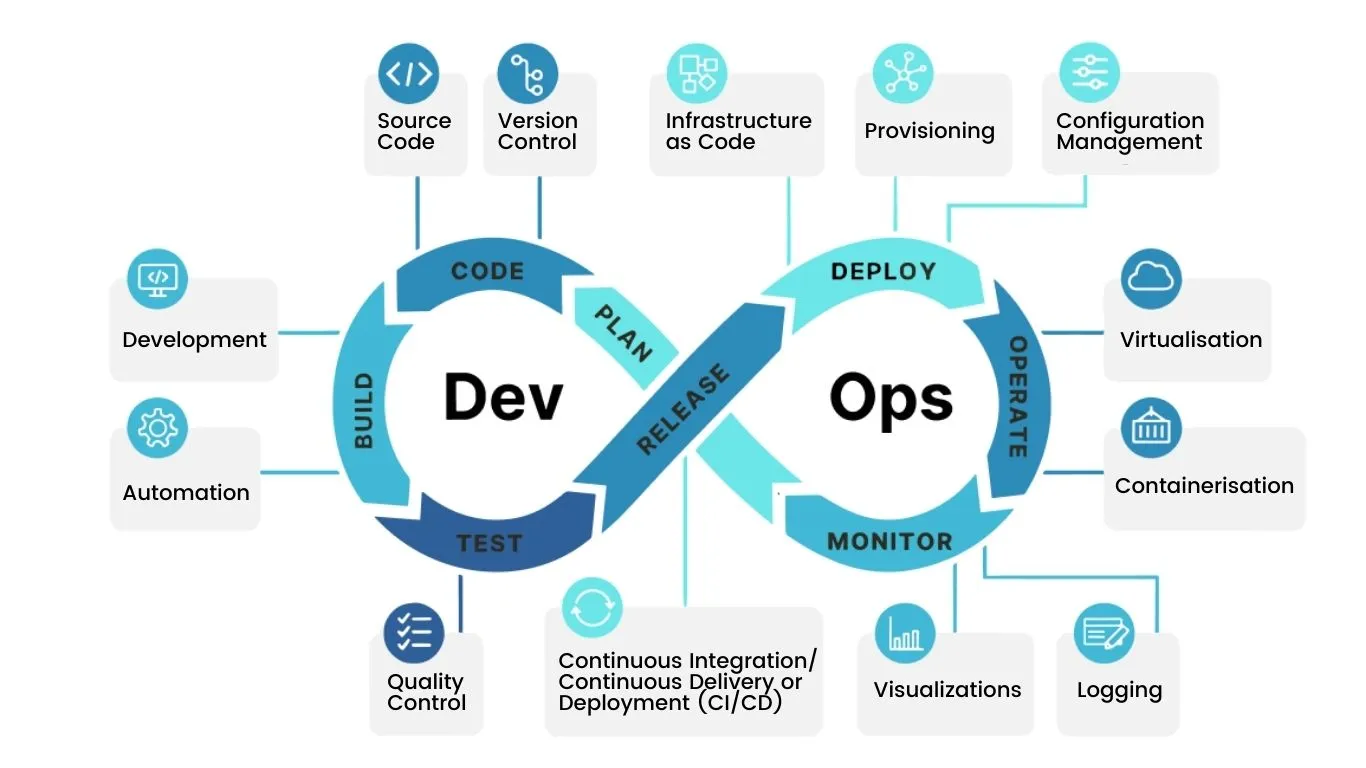
\includegraphics[width=0.85\textwidth]{media/devops-flow}
        \end{center}
    \end{frame}

    \begin{frame}{Стоимость исправления при разработке}
        \begin{center}
            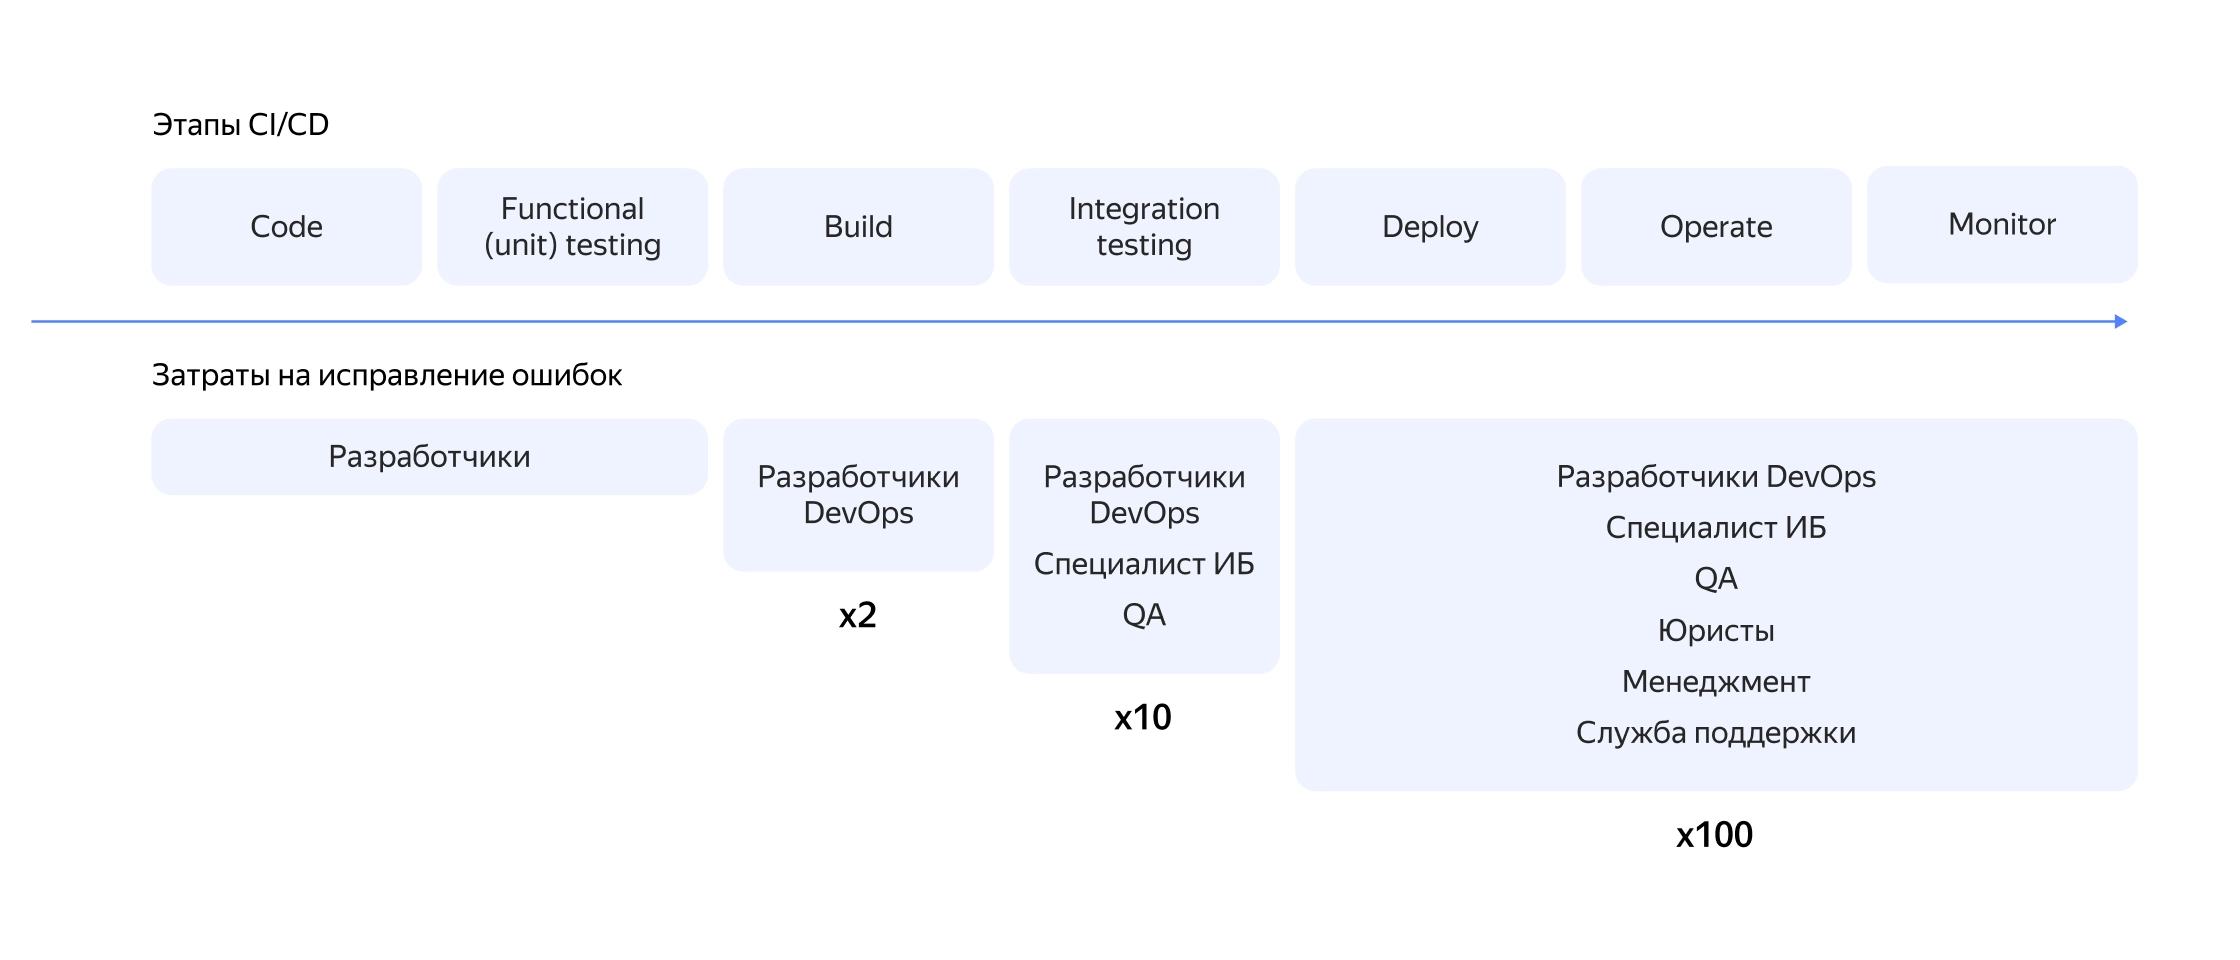
\includegraphics[width=1\textwidth]{media/shift-left}
        \end{center}

        \footnotesize{\textcolor{gray}{\url{https://yandex.cloud/ru/blog/posts/2023/05/devsecops-pipeline}}}
    \end{frame}

    \begin{frame}{Принцип Shift left}
        \begin{center}
            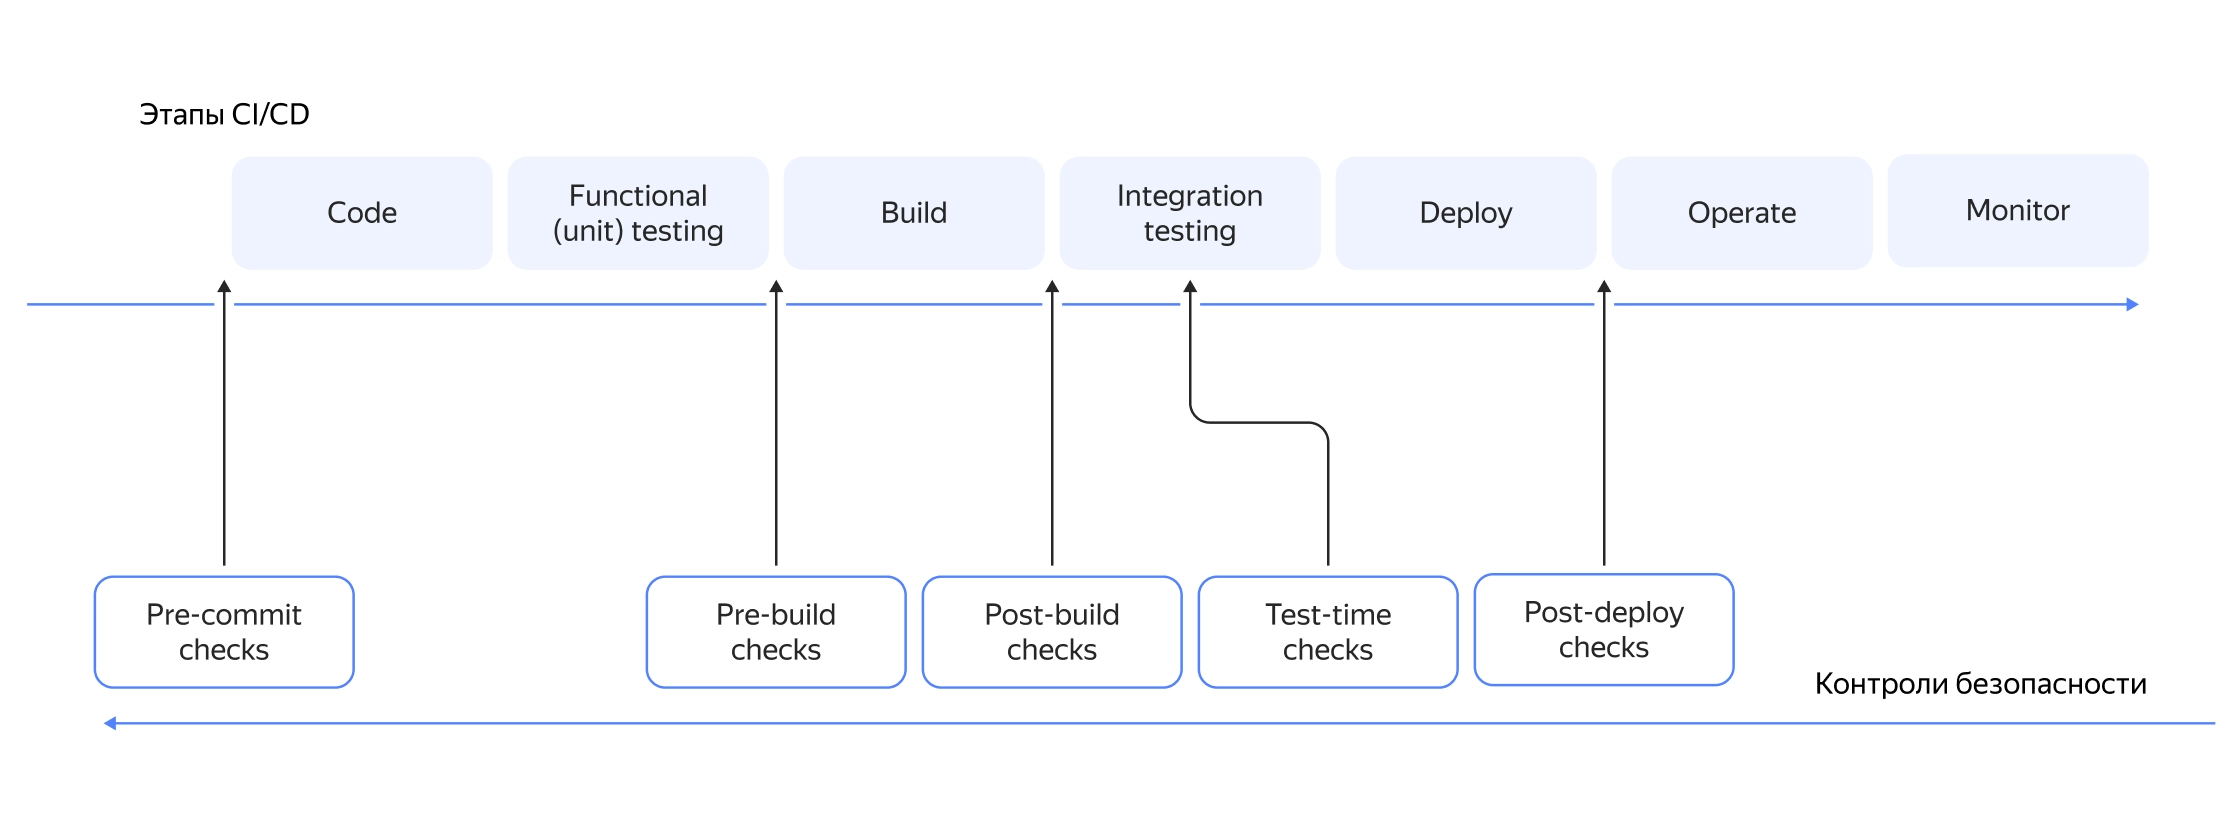
\includegraphics[width=1\textwidth]{media/shift-left-2}
        \end{center}

        \footnotesize{\textcolor{gray}{\url{https://yandex.cloud/ru/blog/posts/2023/05/devsecops-pipeline}}}
    \end{frame}

    \begin{frame}{Модель Secure SDLC}
        \begin{center}
            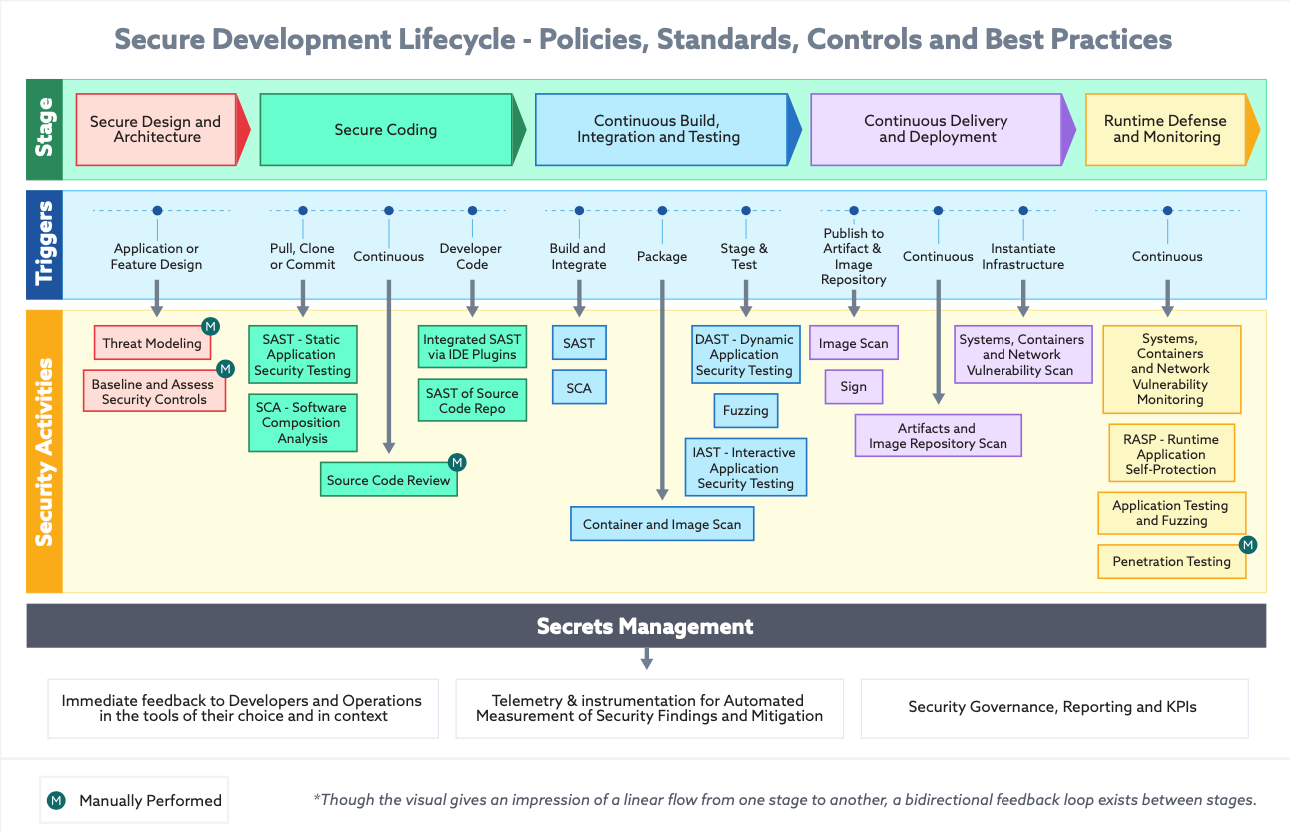
\includegraphics[width=0.72\textwidth]{media/secure-sdlc}
        \end{center}

        \footnotesize{\textcolor{gray}{\url{https://devsecops.pagerduty.com/secure_sdlc/}}}
    \end{frame}

    \begin{frame}{DevSecOps}
        \textbf{DevSecOps - способ организации работы IT команд}

        Включает:
        \begin{itemize}
            \item Все принципы DevOps
            \item Использование проверок безопасности на каждом этапе разработки
        \end{itemize}

        \vspace{0.5cm}

        \textbf{Цель DevSecOps:} быстрая, надежная и \textbf{безопасная} доставка ПО
    \end{frame}

    \begin{frame}{Pre build проверки}
        Secret Detection:
        \vspace{-0.5em}
        \begin{itemize}
            \item \href{https://docs.github.com/en/code-security/secret-scanning/introduction/about-secret-scanning}{GitHub Secret scanning}
            \item \href{https://github.com/zricethezav/gitleaks}{gitleaks}
            \item \href{https://github.com/awslabs/git-secrets}{git-secrets}
        \end{itemize}

        Static Application Security Testing (SAST):
        \vspace{-0.5em}
        \begin{itemize}
            \item \href{https://codeql.github.com/}{CodeQL}
            \item \href{https://www.sonarsource.com/products/sonarqube/server/}{SonarQube}
            \item \href{https://pvs-studio.com/en/pvs-studio/sast/}{PVS Studio}
        \end{itemize}

        Software Composition Analysis (SCA):
        \vspace{-0.5em}
        \begin{itemize}
            \item \href{https://trivy.dev/}{Trivy}
            \item \href{https://github.com/anchore/grype}{Grype}
            \item \href{https://rt-solar.ru/products/solar_appscreener/}{Solar appScreener}
        \end{itemize}
    \end{frame}

    \begin{frame}{Test time проверки}
        Dynamic Application Security Testing (DAST):
        \begin{itemize}
            \item \href{https://www.zaproxy.org/}{OWASP Zed Attack Proxy (ZAP)}
            \item \href{https://global.ptsecurity.com/en/products/ai/}{PT Application Inspector}
            \item \href{https://github.com/awslabs/git-secrets}{git-secrets}
        \end{itemize}

        Interactive Application Security Testing (IAST):
        \begin{itemize}
            \item \href{https://codeql.github.com/}{Synopsys Seeker}
            \item \href{https://global.ptsecurity.com/en/products/ai/}{PT Application Inspector}
        \end{itemize}
    \end{frame}

    \begin{frame}{Post deploy проверки}
        Web Application Firewall (WAF):
        \begin{itemize}
            \item \href{https://www.openappsec.io/}{openappsec}
        \end{itemize}

        Runtime Application Self-Protection (RASP):
        \begin{itemize}
            \item \href{https://github.com/baidu/openrasp}{OpenRASP}
        \end{itemize}
    \end{frame}

    \begin{frame}{Ссылки по теме}
        \begin{itemize}
            \item \url{https://yandex.cloud/ru/training/devsecops}
        \end{itemize}
    \end{frame}
\end{document}